\chapter{Overview of the results and future prospects}\label{ch:overview}

The full analysis setup and the branching fraction measurement results in 
\Cref{sec:partial_branching_fraction_results,sec:total_branching_fraction_results}
are the final result and the ultimate goal of this analysis.
It is the first such implementation of an inclusive radiative analysis at Belle~II.
Moreover, it is the first implementation of a hadronic-tagged \BtoXsgamma measurement since 2007, 
when the result was reported by the BaBar collaboration (see \Cref{tab:btosgamma_inclusive_summary}).
The results of the Belle~II analysis are available in \cite{Belle-II:2022hys}.

This final Chapter is dedicated to the discussion and overview of the results, as well as their significance.
The future prospects of \BtoXsgamma, focusing on the hadronic-tagged measurements, is also discussed.

\section{Discussion of the Belle~II hadronic-tagged \texorpdfstring{\BtoXsgamma}{B->Xs gamma} results}\label{sec:result_discussion}

The resulting values in \Cref{tab:integrated_branching_fractions} are in perfect agreement with the Standard Model values (see \Cref{sec:btosgamma_totalrate_theory}).
They also agree with the past measurements of \BtoXsgamma, which utilise both inclusive and sum-of-exclusive methods.
The visual comparison of all inclusive results is provided in \Cref{fig:measurement_comparison}.
\begin{figure}[htbp!]
    \centering
    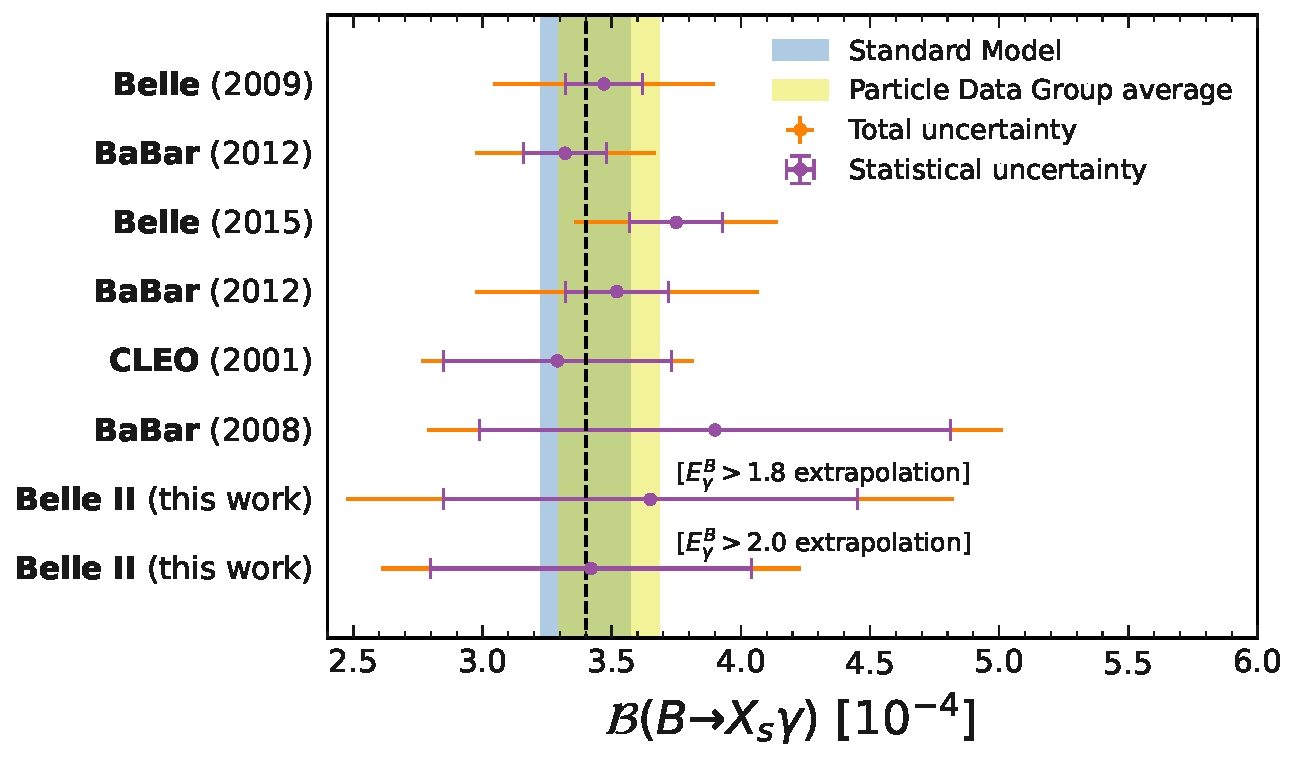
\includegraphics[width=0.45\textwidth]{figures/results_discussion/all_measurements_compared.pdf}
    \caption{\label{fig:measurement_comparison}
        The past measurements of the total branching fraction compared with past results from other experiments.
        The results from other experiments correspond to those in \Cref{tab:btosgamma_inclusive_summary}.
        The results from this analysis are taken from \Cref{tab:integrated_branching_fractions}.
        All values are at their extrapolated values (at $1.6~\gev$ lower energy threshold).
        The Standard Model expectation corresponds to the \Cref{eq:btosgamma_theoretical},
        whereas the Particle Data Group average to \Cref{eq:btosgamma_experimental}.
    }
\end{figure}

The hadronic tagged \BtoXsgamma analysis is dominated statistically, with the systematic components lower, as seen in \Cref{tab:integrated_branching_fractions}.
The systematic uncertainty is larger than the statistical uncertainty only if the lowest-\EB signal-region interval is included in the integrated branching fraction evaluation, 
as the systematic uncertainty is driven by the number of background events in the post-fit sample.

Judging from the partial branching fractions of \BtoXsgamma in \Cref{sec:partial_branching_fraction_results},
the largest contribution to the systematic uncertainty originates from background modelling.
This contribution drops of quickly, as the number of background events decreases.
The \Mbc fitting model uncertainties also drop quickly with \EB, as the main fitting dificulties originate from the contamination of \Mbc distribution by peaking non-\BtoXsgamma events.
On the other hand, the uncertainties due to signal modelling and \BtoXdgamma increase with \EB, as the number of \BtoXsdgamma events grows.

As discussed in \Cref{sec:btosgamma_techniques}, different analysis procedures are complementary to each other.
Therefore, although individually the result is not competetive with the most precise measurements of BaBar and Belle (note that those measurements are performed with $2--3$ times larger datasets),
its results show important consistency between different measurement techniques.
Furthermore, it is a second ever measurement of the hadronic-tagged \BtoXsgamma: therefore it serves as a proof of the measurement technique and its applicability accross different experimental setups.

Consider the hadronic-tagged measurement of BaBar \cite{BaBar:2007yhb} (extrapolated to 1.6~\gev), which obtains:
\begin{equation}\label{eq:babar_measurement}
    \mathcal{B}(\BtoXsgamma) = 3.90 \pm 0.91 \mathrm{(syst.)} \pm 0.64 \mathrm{(stat.)}.
\end{equation}
It is possible to compare this to the results of the analysis presented here (\Cref{tab:integrated_branching_fractions})
to see that the statisitcal uncertainty is ($0.91/0.80\approx=1.14$) times lower.
The improvement of the statistical uncertainty is likely a combination of several reasons:
\begin{itemize}
    \item A higher tagging efficiency at Belle~II offered by the \FEI algorithm compared to the one used at BaBar;
    \item Different continuum suppression strategy (the Belle~II analysis uses a \BDT, whereas BaBar utilised a Fischer discriminant);
    \item Different fitting setup (the Belle~II analysis uses three \PDF{s}, whereas BaBar perform the fit using a Crystal Ball and ARGUS \PDF combination);
\end{itemize}
and others.
\todo[inline]{BaBar tagging efficiency}

For the comparison of systematic uncertainty, it highly depends on the lower-\EB energy threshold.
Therefore, a meaningful comparison is only such where the \EB threshold is the same.
The value in \Cref{eq:babar_measurement} is evaluated with a threshold of $\EB>1.9~\gev$.
Assuming a linear shift of uncertainty, the results of this analysis are averaged $0.5\cdot(0.52+0.86)\approx0.69$.
Therefore, the systematic uncertainty is slightly higher but comparable.
Furthermore, the uncertainty estimates at this stage can still be improved
(see \todo{seee})

\section{Future prospects for hadronic-tagged \texorpdfstring{\BtoXsgamma} analysis at Belle~II}\label{sec:future_prospects}

Belle~II is an ongoing experiment, which means that more and more \epem collision data will be recorded in the next decade.
No other ongoing experiment is able to contribute to the inclusive radiative measurements.
As it is clear from \Cref{sec:results} and \Cref{sec:result_discussion}, at the moment the analysis is limited statistically.
With the larger Belle~II dataset, the importance of systematic effects will grow.
Although in this analysis several systematic uncertainties are set at their conservative estimates (see \Cref{sec:background_normalisation_systematic}, \Cref{sec:xdgamma_systematic} etc.),
additional studies will allow to reduce them.
This was studied (as part of original work for this thesis), and the results are available in \cite{Belle-II:2022cgf}.
The uncertainty projections for the hadronic-tagged \BtoXsgamma are summarised in \Cref{tab:btosgamma_projections}.

\begin{table}[htbp!]
    \caption{\label{tab:btosgamma_projections}
    The projected uncertainties for the hadronic-tageed \BtoXsgamma with the increased Belle~II data set size.
    These projections are evaluated assuming the principal contributions in systematic uncertainty arise from
    background modelling and suppression uncertainties.
    The baseline case is presented for a scenario where the remaining good background of good tag-\B mesons is known to $10\%$,
    whereas the improved scenario where it is known to $5\%$.
    }
    \begin{tabular}{cccccc}
        \multirow{2}{*}{Lower \EB threshold} & \multicolumn{4}{c}{Statistical uncertainty} & \multirow{2}{*}{\makecell{Baseline (improved)\\ systematic uncertainty}} \\
        & 1~\invab& 5~\invab & 10~\invab & 50~\invab & \\
        \hline
        1.4~\gev & 10.7\% & 6.4\% & 4.7\% & 2.2\% & 10.3 \% (5.2\%)\\
        1.6~\gev & 9.9 \% & 6.1\% & 4.5\% & 2.1\% & 8.5 \% (4.2\%)\\ 
        1.8~\gev & 9.3 \% & 5.7\% & 4.2\% & 2.0\% & 6.5 \% (3.2\%)\\ 
        2.0~\gev & 8.3 \% & 5.1\% & 3.8\% & 1.7\% & 3.7 \% (1.8\%)\\ 
    \end{tabular}
\end{table}

The statistical uncertainties for the hadronic tagged \BtoXsgamma are expected to reach $5\%$ level with $5~\invab$ of Belle~II data.
The systematic uncertainty expectations are evaluated assuming that the main contributor to the systematic uncertainty
is the remaining-\BB background subtraction and \FEI tagging.
If the knowledge of remaining-\BB background stays at the 10\% level ($8.7\%$ evaluated in this analysis) and \FEI calibration uncertainty is not improved,
it is expected that a 6.5\% total systematic uncertainty on the branching fraction of \BtoXsgamma can be achieved.
On the other hand, if remaining after-fit \BB backgrounds are understood to a $5\%$ level it is plausible half the expected systematic uncertainty.
The uncertainties on signal selection efficiency will further reduce as the understanding of background suppression tools (e.g. the \piz veto, \ZMVA) improves.
The \BtoXdgamma in the future will be accurately subtracted when precise \BtoXdgamma measurements with Belle~II are performed.


Summarising, it is plausible to expect world-leading hadronic-tagged \BtoXsgamma measurements when Belle~II has collected $1-5~\invab$ of data.
Indeed, other type of inclusive \BtoXsgamma analysis techniques are already systematically limited (see \Cref{tab:btosgamma_inclusive_summary}) with the Belle and BaBar datasets.
Therefore, a different approach, one that will be provided by the hadronic-tagged analyses, is necessary for further insights in the radiative \BtoXsgamma transitions.
In the short term, as Belle has not reported a hadronic-tagged \BtoXsgamma analysis, a joint Belle and Belle~II may provide a total dataset of approximately $1\invab$, making such results achievable in the next couple of years.

\section{Input of the results to theoretical averages}\label{sec:input_to_theory}

\todo[inline]{Misiak, Kerstin results if I ever get them...}